
\begin{figure}

    \centering
    \textbf{MATLAB}\hspace{8em}
    \textbf{Original}\hspace{8em}
    \textbf{Python}
    

    \begin{subfigure}{\textwidth}
        \centering
        
        \textbf{\rotatebox[origin=c]{90}{RMHL}}\begin{subfigure}{\textwidth}
        \centering
        
        \hspace{-1em}
        \includegraphics[trim=3cm 0.5cm 3cm 4cm, clip=true, height=.25\linewidth]{Figures/Fig_T4/MATLAB/RMHL_T3_Trajectory.eps}
        \hspace{3em}
        \includegraphics[trim=1cm 0cm 1cm 0cm, clip=true,scale=0.5,
        height=.25\linewidth]{Figures/Fig_T4/Orig/RMHL_T3_Trajectory.png}
        \hspace{3em}
        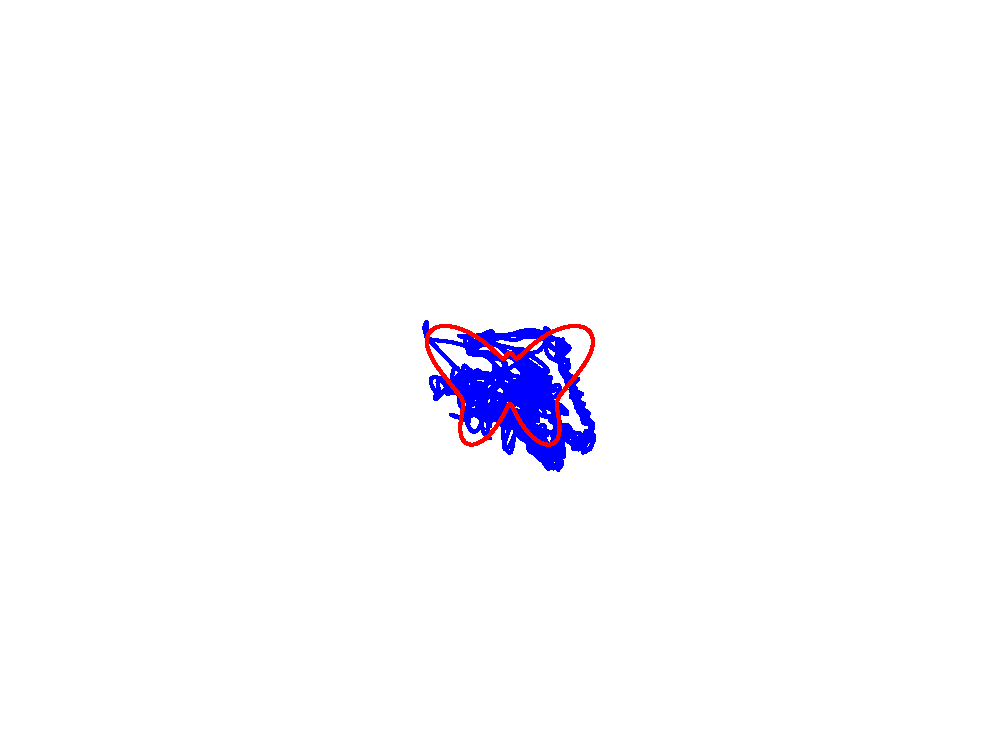
\includegraphics[trim=6cm 4.5cm 6cm 3cm, clip=true,  height=.25\linewidth]{Figures/Fig_T4/Python/RMHL_T3_Trajectory.eps}
        
        \end{subfigure}
         
        
        
    \caption{Results for Task 3 with the RMHL algorithm, using the default seed (5489) for the random number generator. The target trajectory is imitated well by the model during the training phase (not shown), however, it poorly maintains the time-series during the testing phase, in both implementations, as presented in \cite{pyle2019}.}
    \label{Fig:compTask3RMHL}
    \end{subfigure}
    
    \begin{subfigure}{\textwidth}
        \centering
        
        \textbf{\rotatebox[origin=c]{90}{SUPERTREX}}\begin{subfigure}{\textwidth}
        \centering
        
        \hspace{0em}
        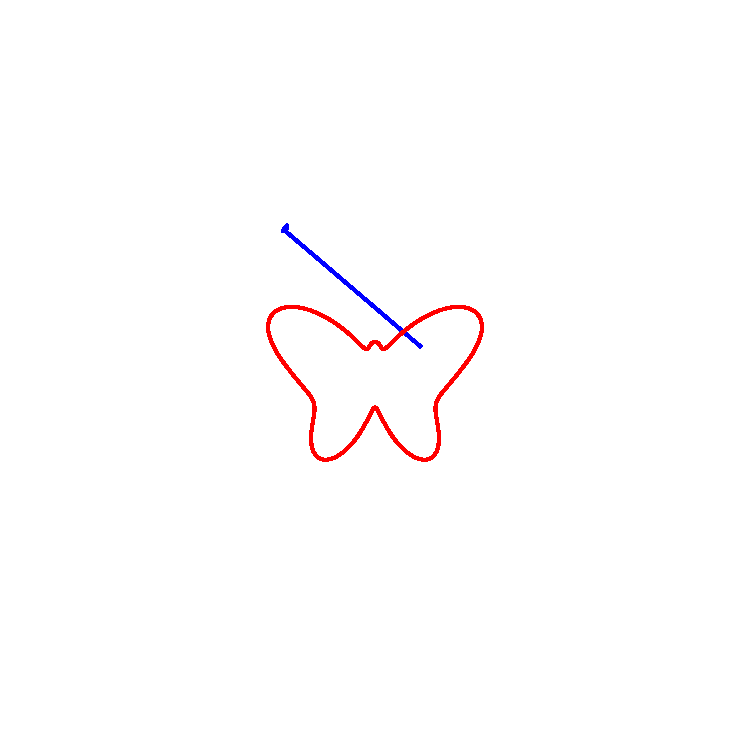
\includegraphics[trim=4cm 4.25cm 4cm 3.5cm, clip=true, height=.2\linewidth]{Figures/Fig_T4/MATLAB/ST_T3_Trajectory.eps}
        \hspace{2em}
        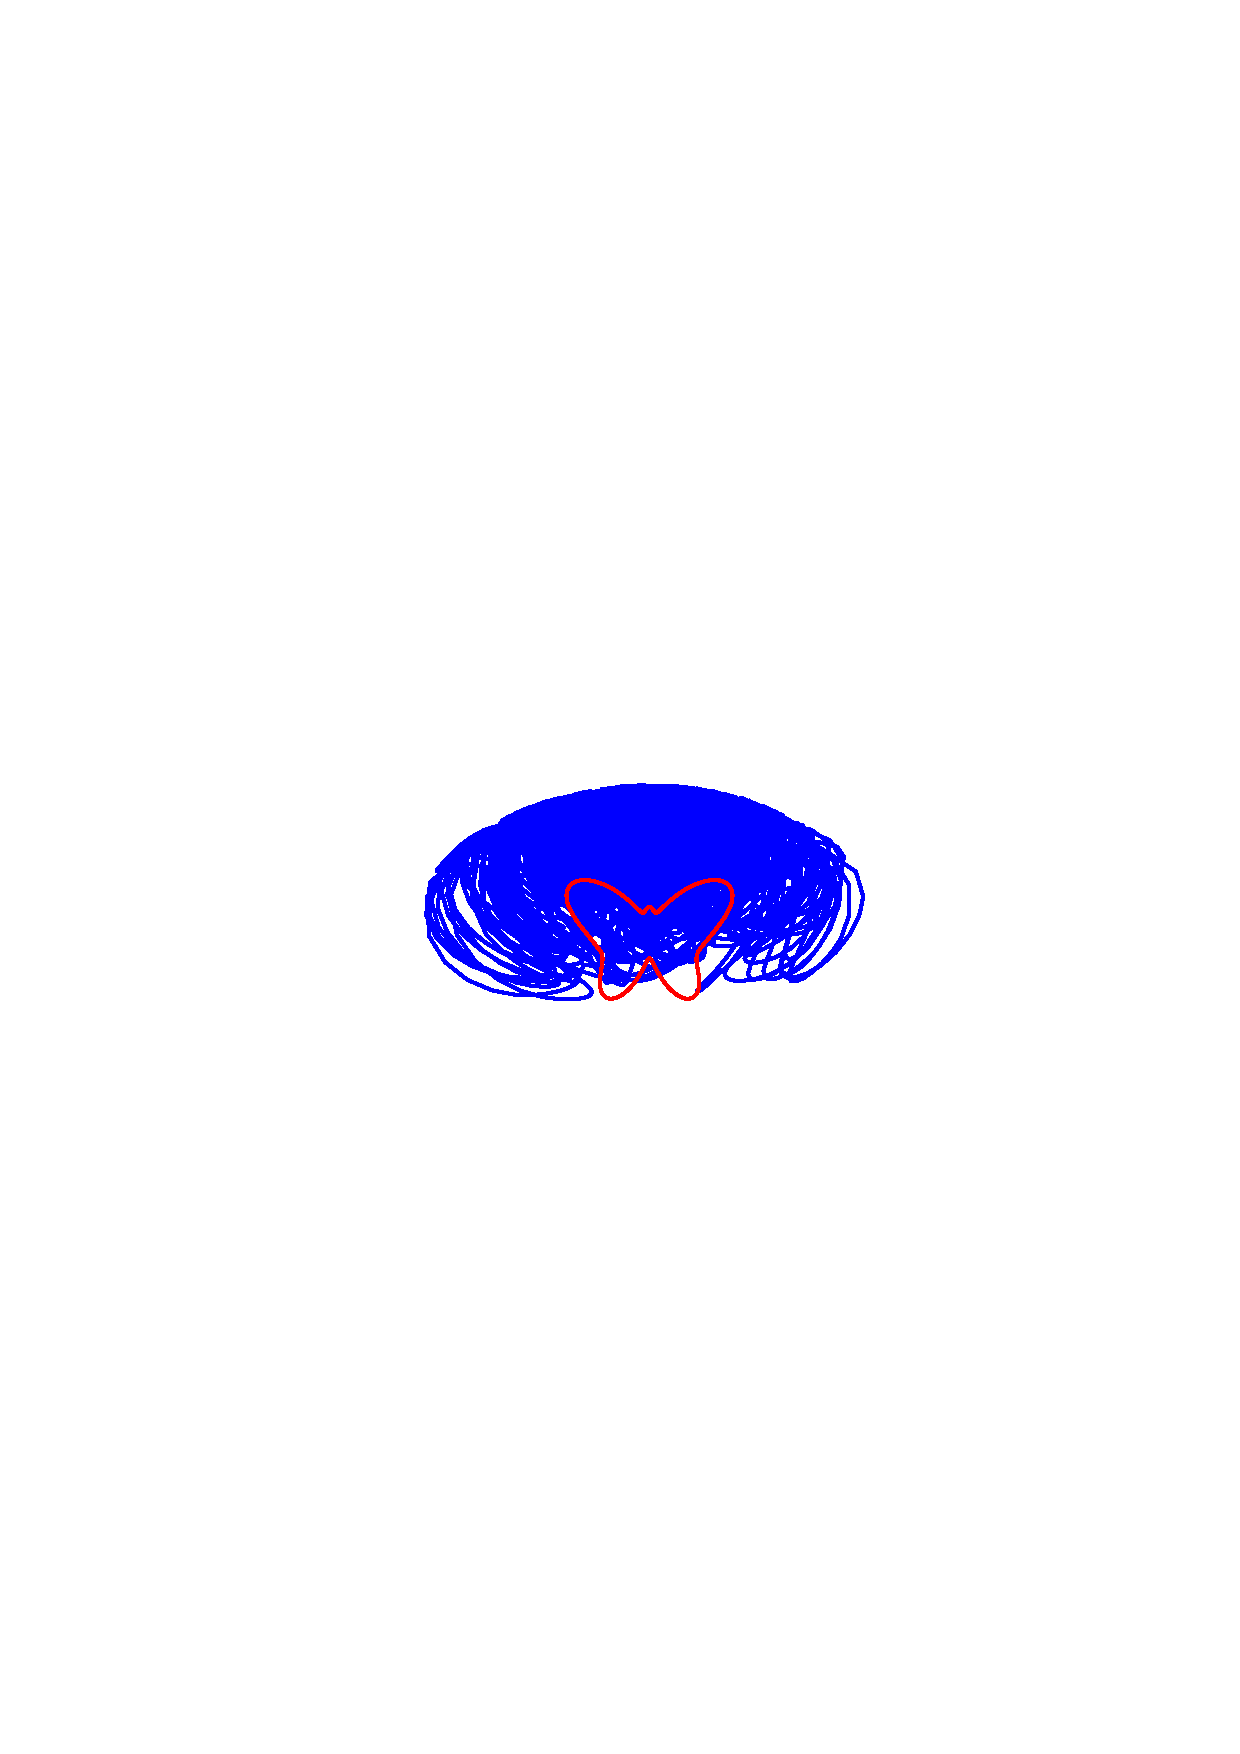
\includegraphics[trim=0cm 0cm 1cm 0cm, clip=true, height=.15\linewidth]{Figures/Fig_T4/Orig/ST_T3_Trajectory.png}
        \hspace{-.25em}
        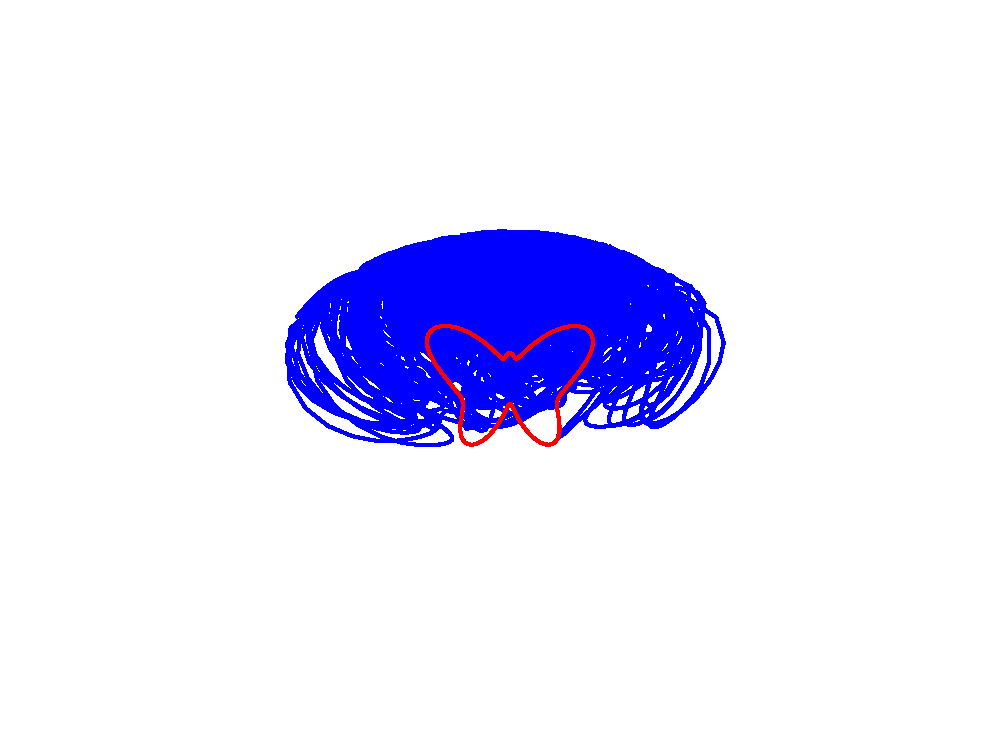
\includegraphics[trim=4cm 4.75cm 4cm 3.5cm, clip=true,  height=.2\linewidth]{Figures/Fig_T4/Python/ST_T3_Trajectory.eps}
        \hspace{-3em}
        
        \end{subfigure}
        
        
        \textbf{\rotatebox[origin=c]{90}{$\theta_1$}}\begin{subfigure}{\textwidth}
        \centering
        
        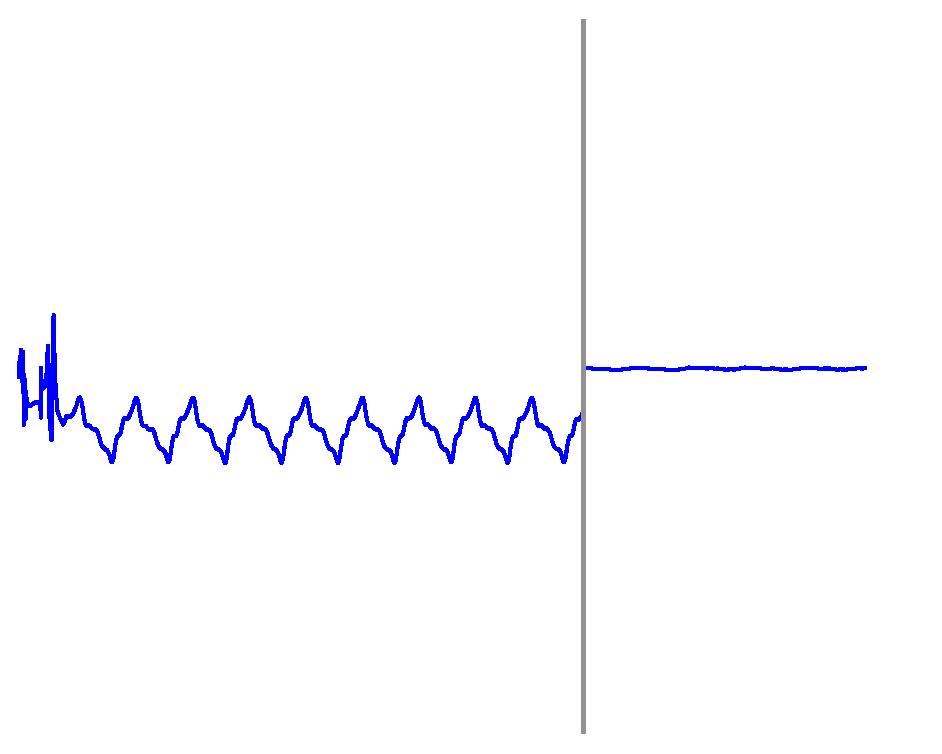
\includegraphics[height=0.1\linewidth,width=.45\linewidth]{Figures/Fig_T4/MATLAB/ST_T3_Theta0.eps}
        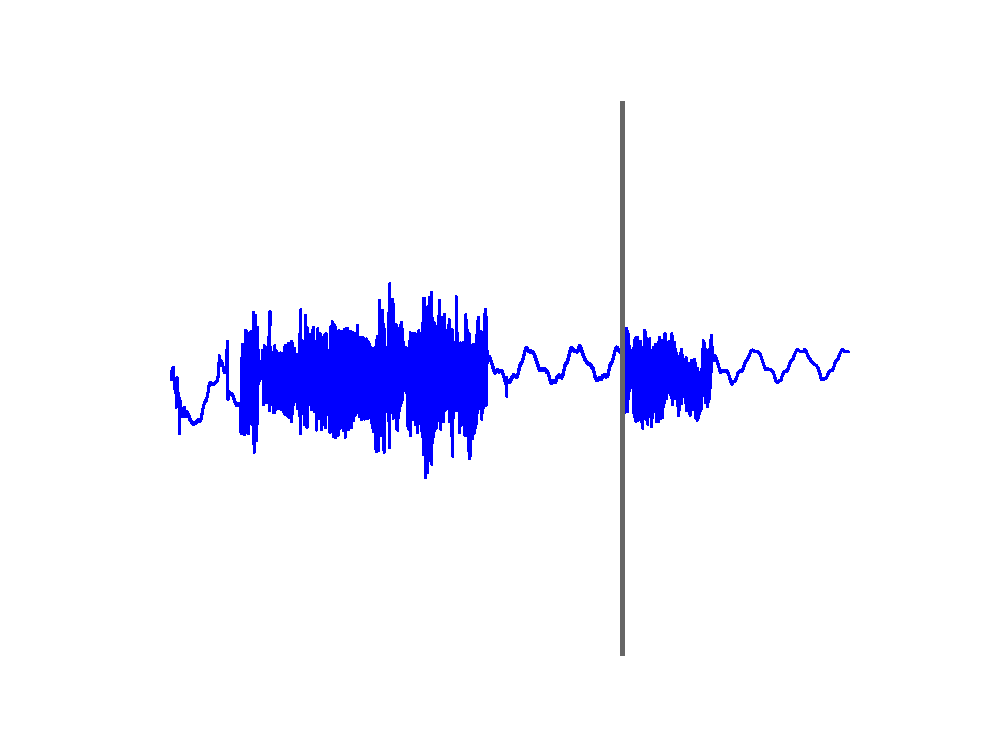
\includegraphics[trim=2cm 1cm 2cm 1cm, clip=true, height=0.1\linewidth,width=.45\linewidth]{Figures/Fig_T4/Python/ST_T3_Theta0.eps}
        
        \end{subfigure}
        
        
        \textbf{\rotatebox[origin=c]{90}{$\theta_2$}}\begin{subfigure}{\textwidth}
        \centering
        
        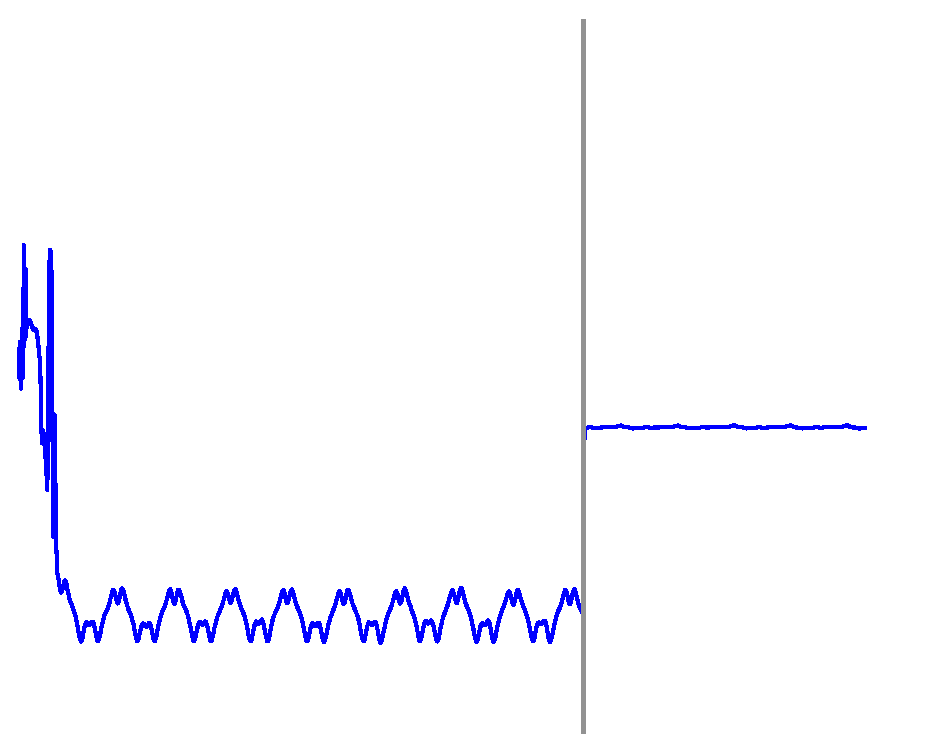
\includegraphics[height=0.1\linewidth,width=.45\linewidth]{Figures/Fig_T4/MATLAB/ST_T3_Theta1.eps}
        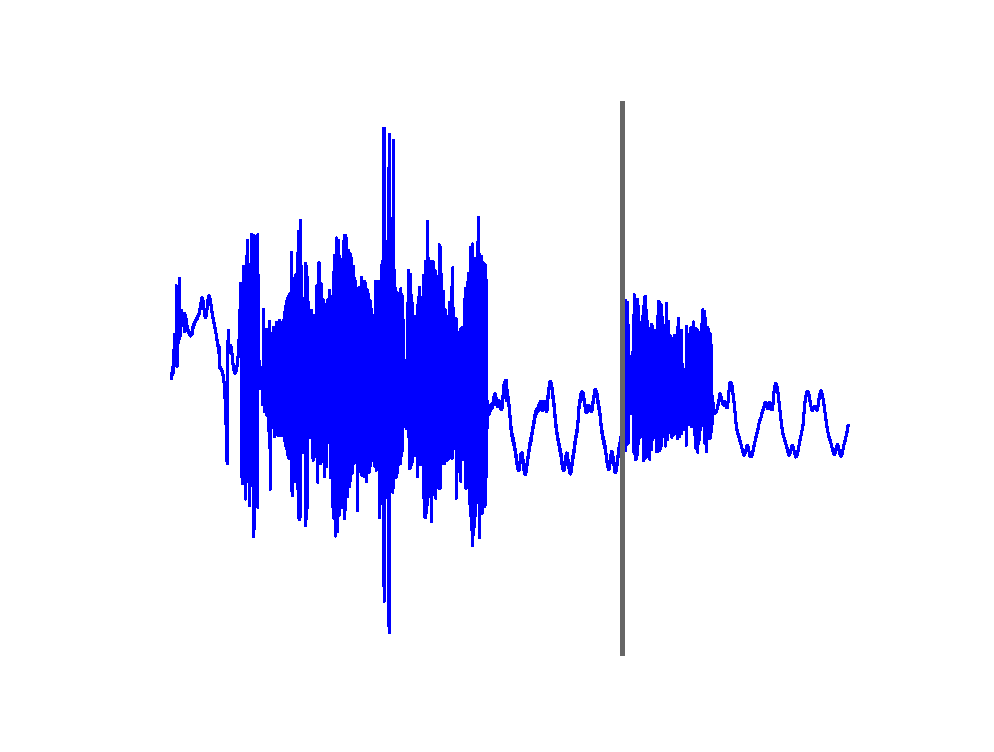
\includegraphics[trim=2cm 1cm 2cm 1cm, clip=true,height=0.1\linewidth,width=.45\linewidth]{Figures/Fig_T4/Python/ST_T3_Theta1.eps}
        
        \end{subfigure}
        
        
        \textbf{\rotatebox[origin=c]{90}{$\theta_3$}}\begin{subfigure}{\textwidth}
        \centering
        
        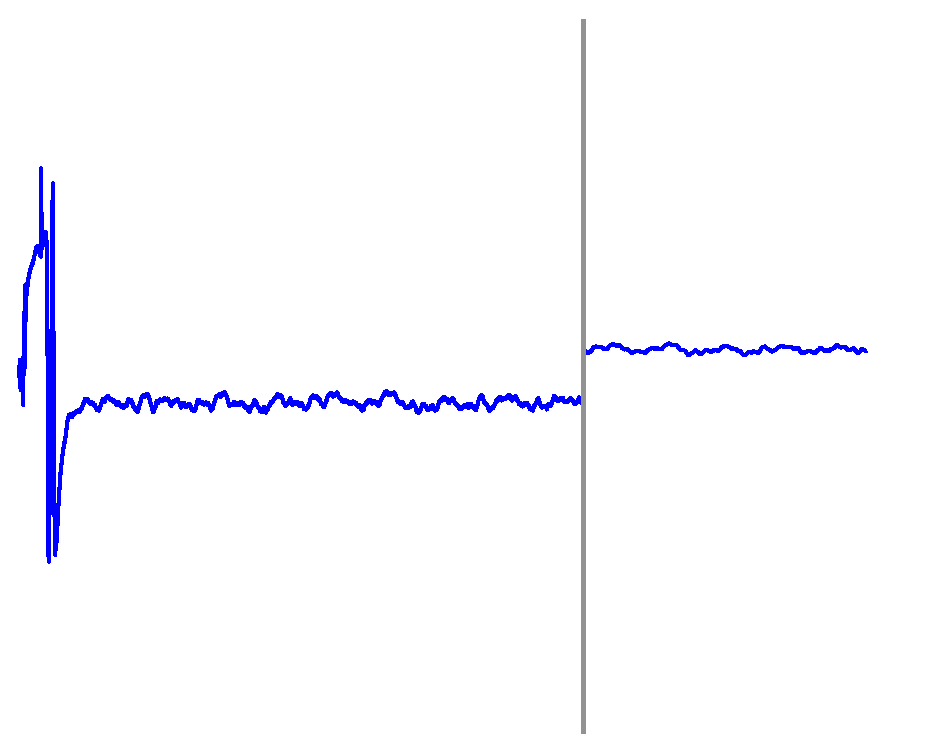
\includegraphics[height=0.1\linewidth,width=.45\linewidth]{Figures/Fig_T4/MATLAB/ST_T3_Theta2.eps}
        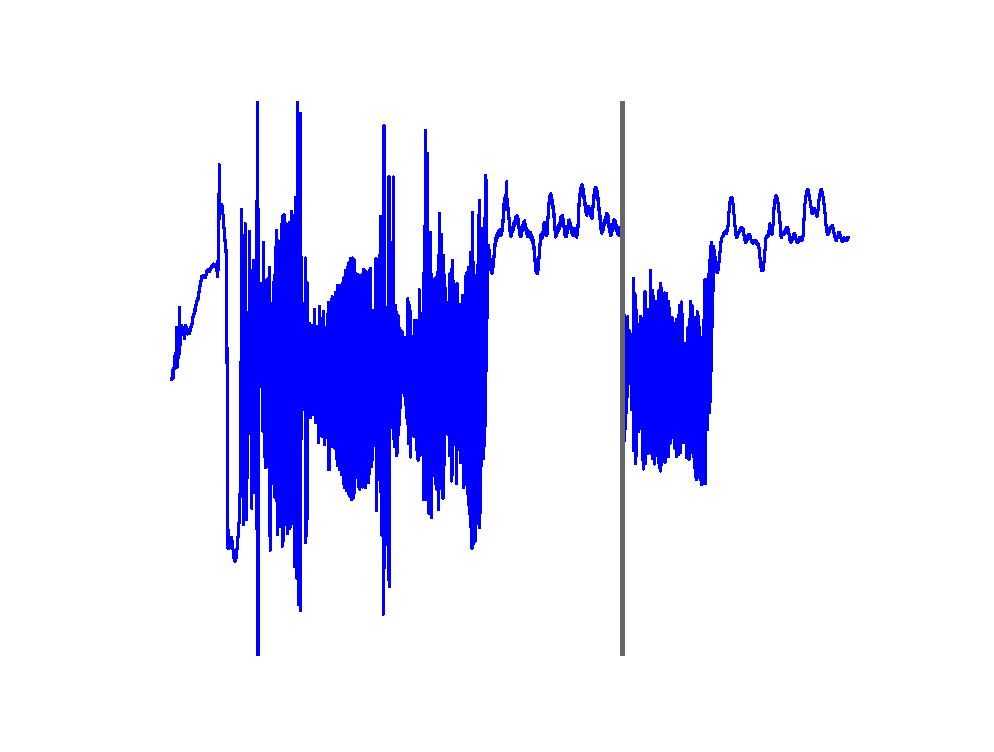
\includegraphics[trim=2cm 1cm 2cm 1cm, clip=true,height=0.1\linewidth,width=.45\linewidth]{Figures/Fig_T4/Python/ST_T3_Theta2.eps}
        
        \end{subfigure}
        
        
        \textbf{\rotatebox[origin=c]{90}{MSE}}\begin{subfigure}{\textwidth}
        \centering
        
        \hspace{-1.9em}
        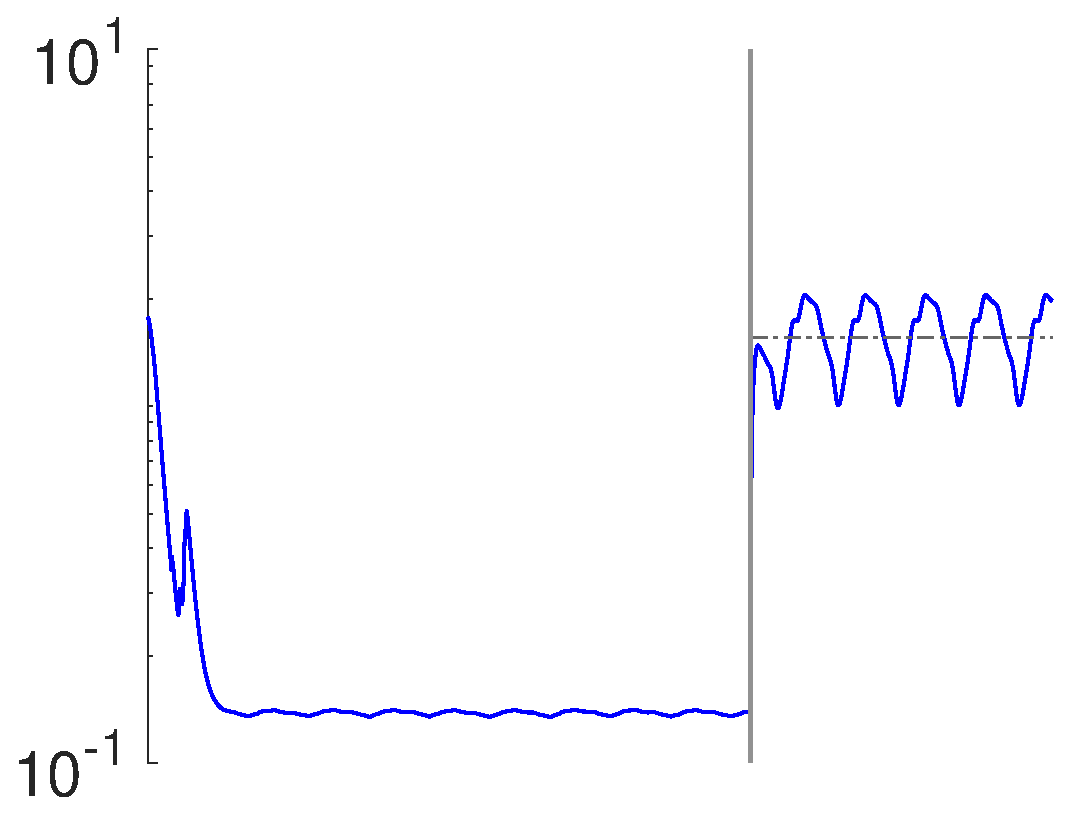
\includegraphics[height=0.2\linewidth,width=.45\linewidth]{Figures/Fig_T4/MATLAB/ST_T3_MSE.eps}
        \hspace{.75em}
        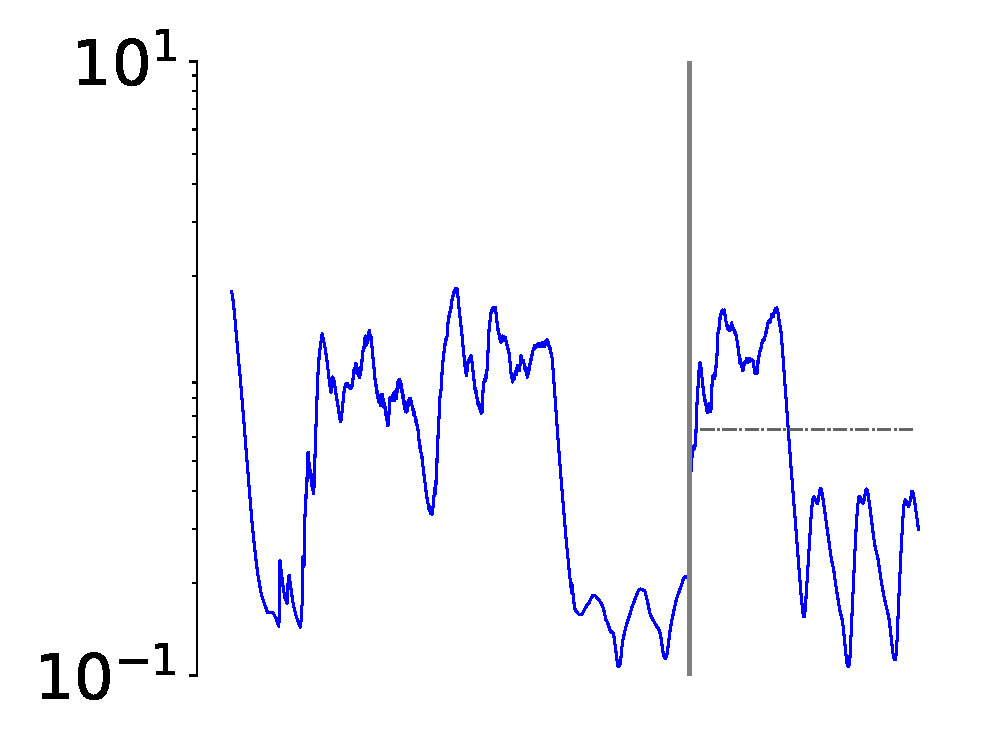
\includegraphics[height=0.2\linewidth,width=.45\linewidth]{Figures/Fig_T4/Python/ST_T3_MSE.eps}
        
        \end{subfigure}
        
        
        
        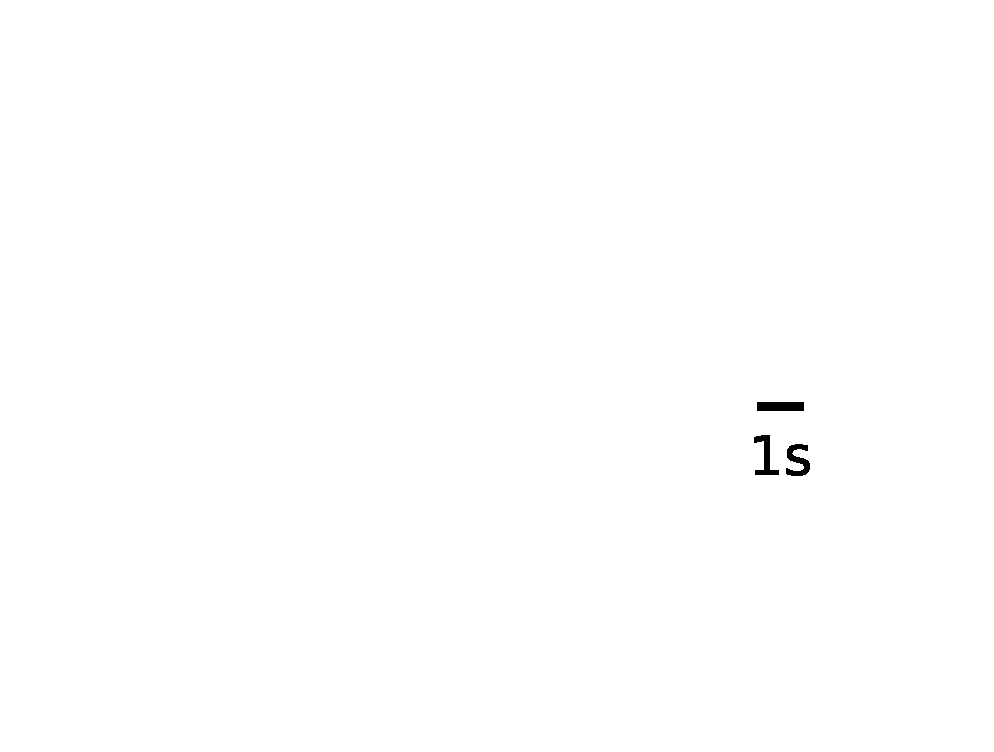
\includegraphics[trim=2cm 6cm 2cm 6cm, clip=true,height=0.05\linewidth,width=.4\linewidth]{Figures/Fig_T1/Python/ST_T1_Scale.eps}
        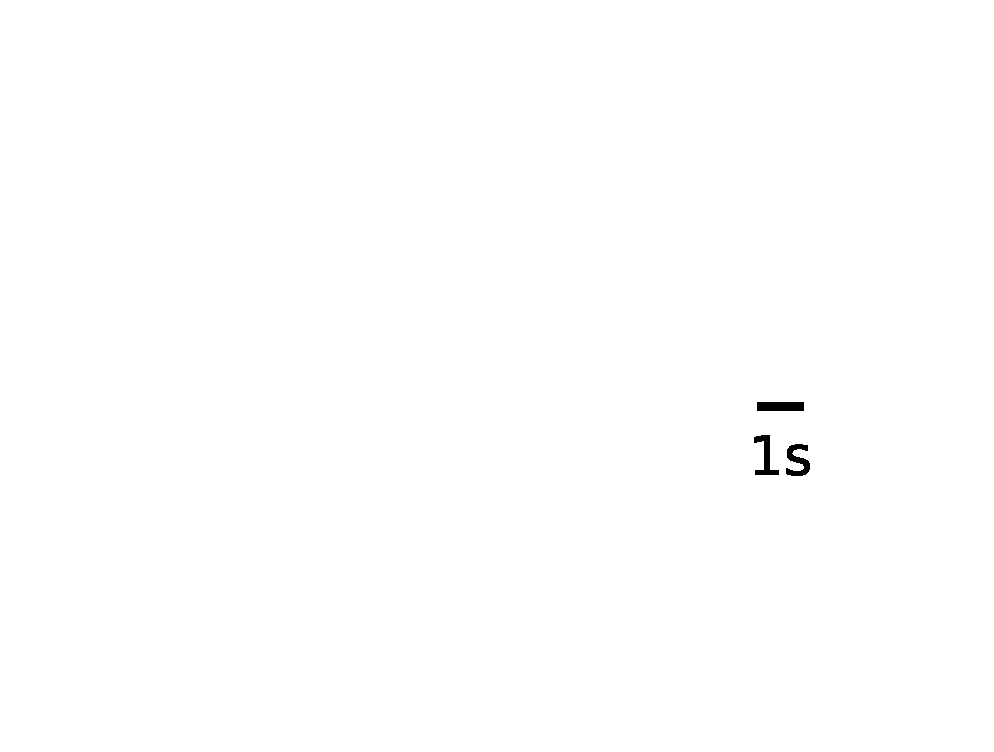
\includegraphics[trim=2cm 4cm 2cm 6cm, clip=true,height=0.05\linewidth,width=.45\linewidth]{Figures/Fig_T1/Python/ST_T1_Scale.eps}
        

    \caption{Results for Task 3 with the SUPERTREX algorithm using the default seed (5489) for the random number generator. The target time‐series is learned accurately during the training phase, but is not maintained during the testing phase, in both implementations, in contrast to the results presented in \cite{pyle2019}.}
    \label{Fig:compTask3ST}
    
    \end{subfigure}
    
    \begin{subfigure}{\textwidth}
        \centering
        
        \textbf{\rotatebox[origin=c]{90}{SUPERTREX}}\begin{subfigure}{\textwidth}
        \centering
        
        
\includegraphics[trim=4cm 4.25cm 4cm 4.75cm, clip=true, height=.2\linewidth]{Figures/Fig_T4/MATLAB/ST_T3_Trajectory_295728336.eps}
        \hspace{1em}
        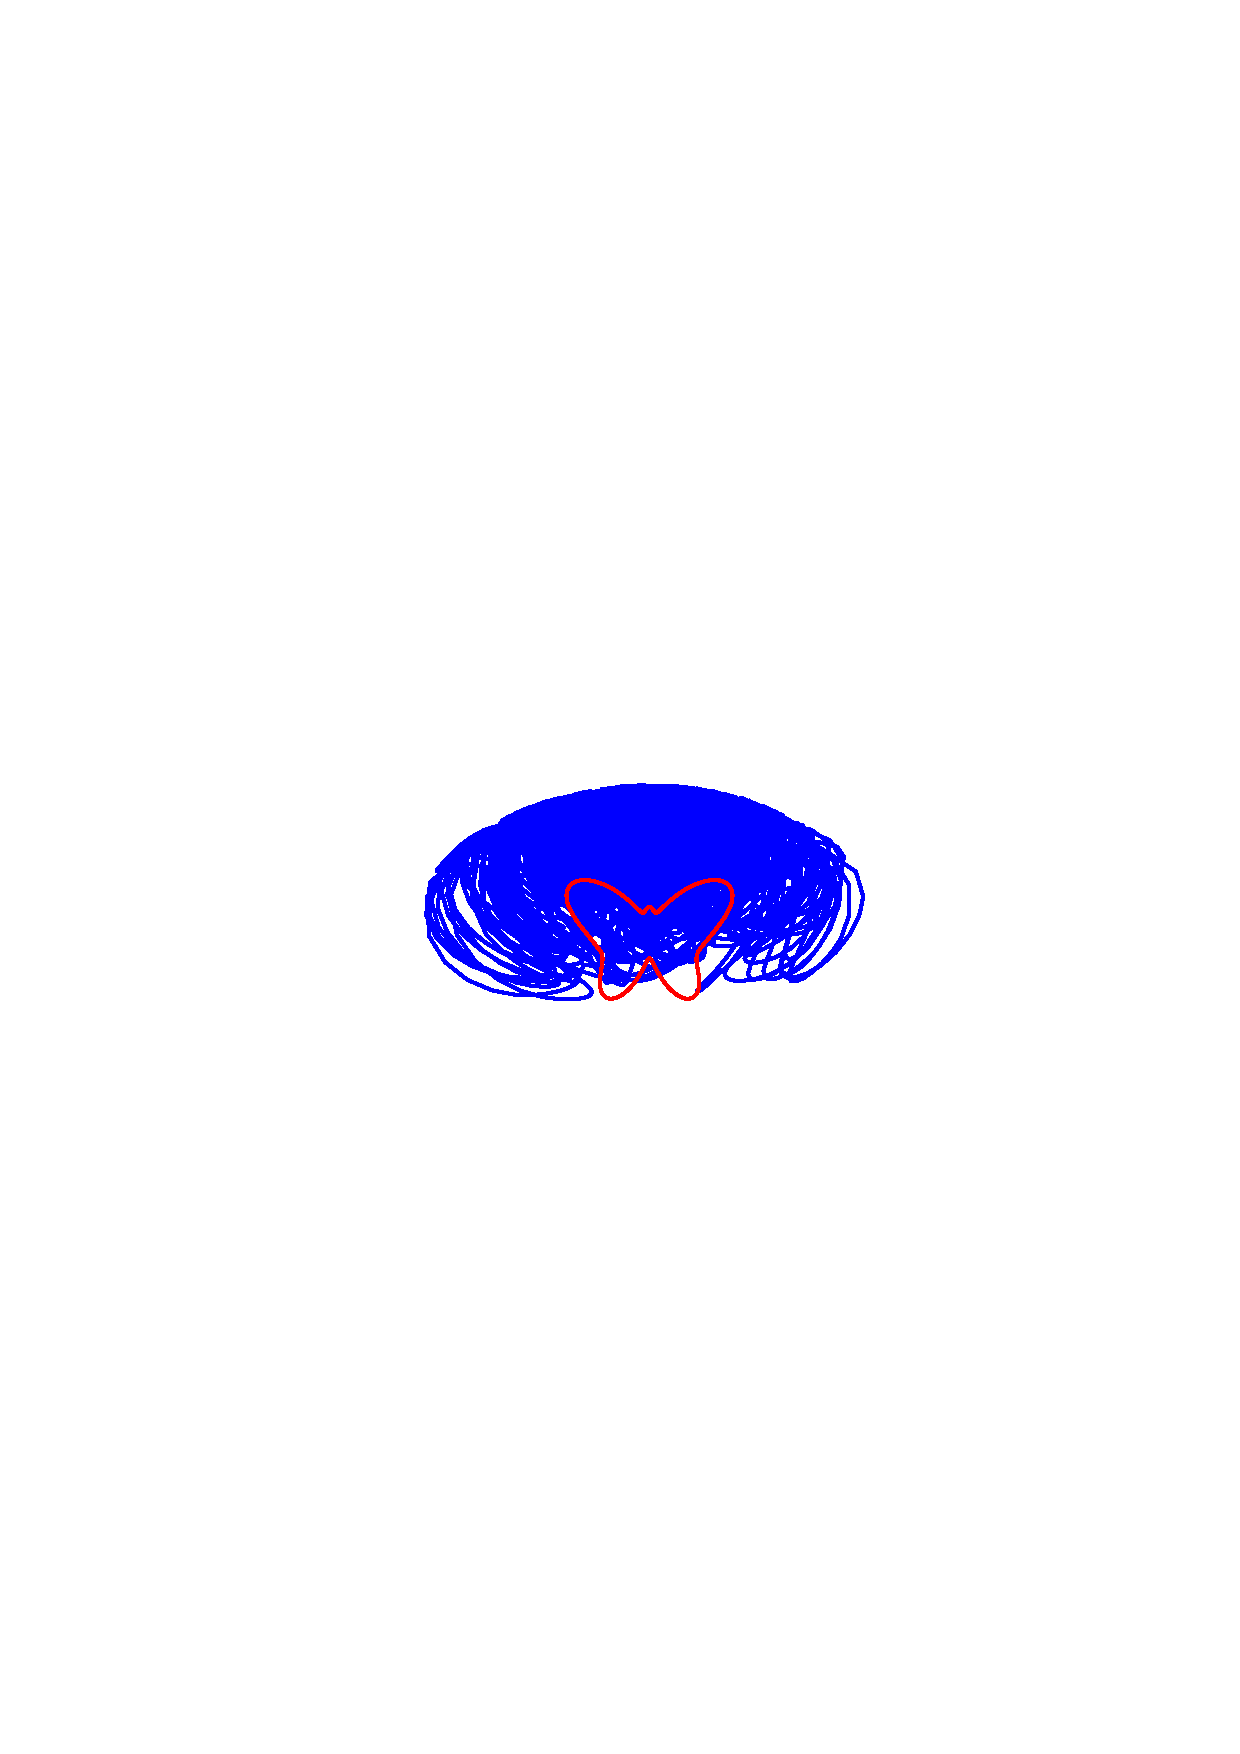
\includegraphics[height=.2\linewidth]{Figures/Fig_T4/Orig/ST_T3_Trajectory.png}
        \hspace{1em}
        
\includegraphics[trim=6.5cm 4.75cm 6.5cm 5cm, clip=true,  height=.2\linewidth]{Figures/Fig_T4/Python/ST_T3_Trajectory_5624282.eps}
        
        \end{subfigure}
        

    \caption{Results for Task 3 with the SUPERTREX algorithm using different implementations (MATLAB, left and Python adaptation, right) and different seeds (295728336, left and 5624282, right) for the random number generator. The target trajectory is learned accurately during the training phase, and is also maintained in a stable manner, with slight divergences (Deviation: 295728336: $0.215\pm0.073$; 5624282: $0.190\pm0.054$) , during the testing phase, in both implementations, similar to the results presented in \cite{pyle2019}.}
    \label{Fig:compTask3STrseeed2}
    
    \end{subfigure}

        
\caption{Comparison of the performances of original scripts (left column) and Python adaptation (right column) with the results presented in the original article (center column), for RMHL and SUPERTREX, on Task 3 \cite{pyle2019}. Each subfigure shows the target trajectory (red) with the trajectory generated by the algorithm (blue) throughout the test phase. In the second subfigure, the the middle rows show the time-series (blue) generated by the model (joint angles ($\theta_i$), in this case). The bottom row shows the distance from target metric (blue) over the simulation (x and y coordinates, in this case), using the log scale for the y axis.  The horizontal grey line, in the test phase, indicates the deviation metric. The grey vertical line marks the separation of the training and testing phase.}
\label{Fig:Comparison_Task3}

\end{figure}